In section 1, 2, we present the result of convergence in both h
refinement and p refinement with the following steady-state
Poisson differential equation:
\begin{equation*}
    \frac{d^2}{dx^2} u(x) = \sin(\pi x),
\end{equation*}
for all x in $[0, 1]$.


\subsection {H-Convergence of 1-D Spectral Method}

This test is to validate the relation between size of element and
the accuracy of approximation. We apply equidistance element and
investigate the movement of error scale. As shown in Figure
\ref{sinDDhconv} and \ref{sinDNhconv}, the smaller are the
elements, the more exact is the solution. Moreover by testing with
different order of basis, we also could see the fact that the
higher are orders, the faster do they converge.


\begin{itemize}

\item Dirichlet-Dirichlet Case
\begin{figure}[h]
\begin{center}
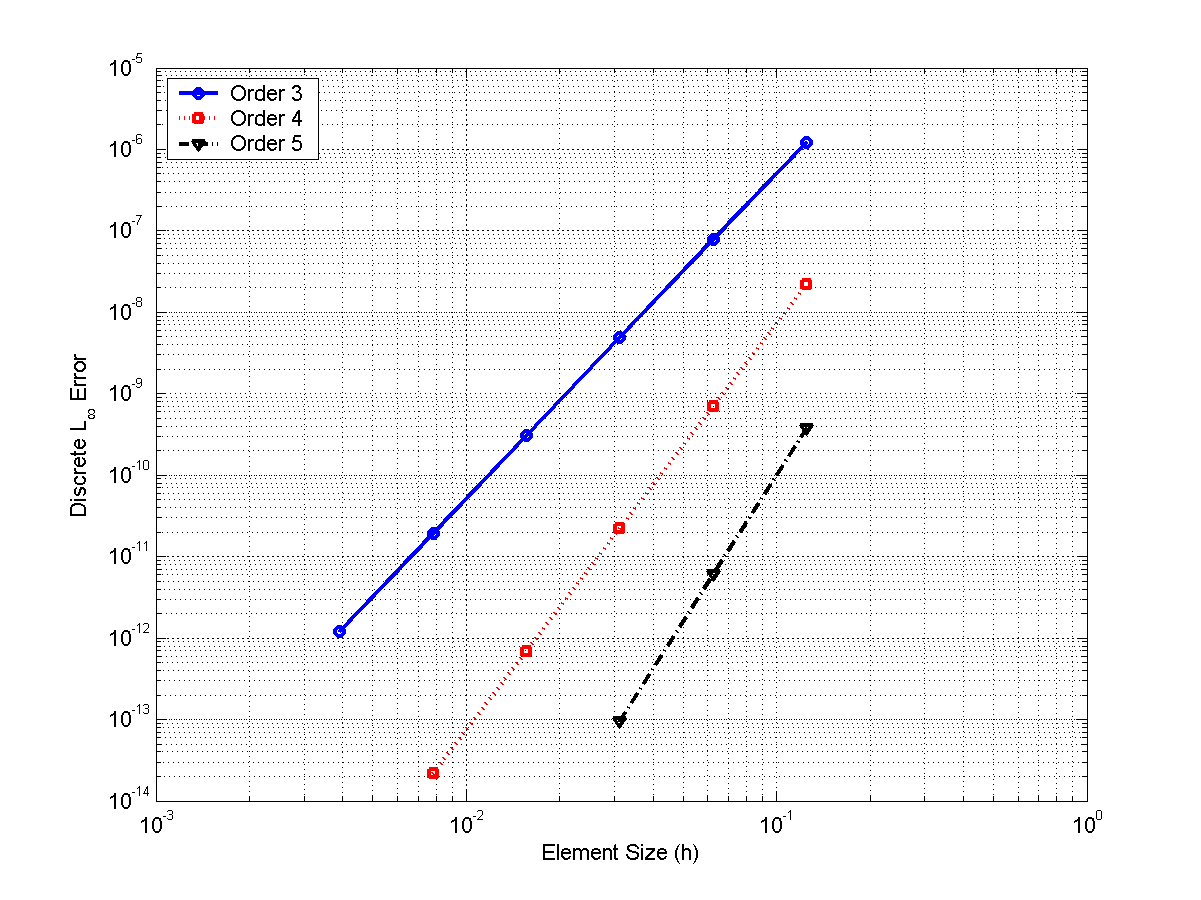
\epsfig{file = figs_dd/sinDDhconv.eps, %
        height = 9cm}
\caption{\label{sinDDhconv}Graph showing change of errors by the
increase of the number of elements: Dirichlet-Dirichlet}
\end{center}
\end{figure}

\begin{table}[h]
\centering \caption{\label{hconv1t} Specification of
                              Figure\ref{sinDDhconv} and their errors}
\begin{tabular}{|c|c|c|} \hline
Polynomial order&Error&Slope   \\ \hline \hline
    3&$1.1940e-012$ &$3.9946$ \\ \hline
    4&$2.2204e-015$ &$4.9875$ \\ \hline
    5&$2.4147e-015$ &$5.9839$ \\ \hline
\end{tabular}
\end{table}

\item Dirichlet-Neumann Case


\begin{figure}[h]
\begin{center}
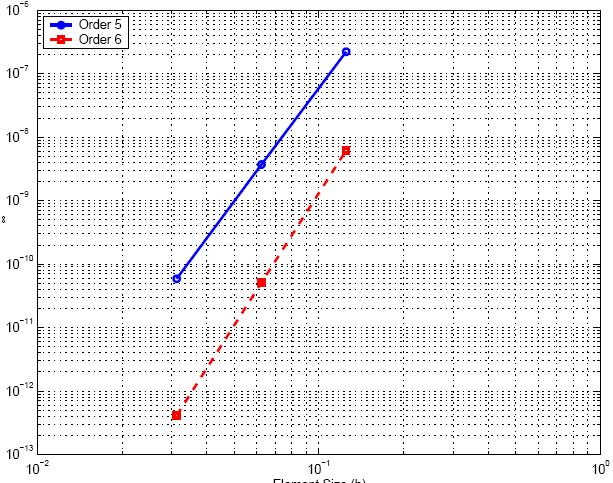
\epsfig{file = figs_dn/sinDNhconv.eps, %
        height = 9cm}
\caption{\label{sinDNhconv}Graph showing change of errors by the
increase of the number of elements: Dirichlet-Dirichlet}
\end{center}
\end{figure}

\begin{table}[h]
\centering \caption{\label{hconv2t} Specification of
                              Figure\ref{sinDNhconv} and their errors}
\begin{tabular}{|c|c|c|} \hline
Polynomial order&Error&Slope   \\ \hline \hline
    3&$1.1620e-012$ &$4.0024$ \\ \hline
    4&$4.6629e-014$ &$4.9877$ \\ \hline
    5&$9.7367e-014$ &$5.9775$ \\ \hline
\end{tabular}
\end{table}


\end{itemize}



\subsection {P-Convergence of 1-D Spectral Method}



\begin{itemize}

\item Dirichlet-Dirichlet Case
\begin{figure}[h]
\begin{center}
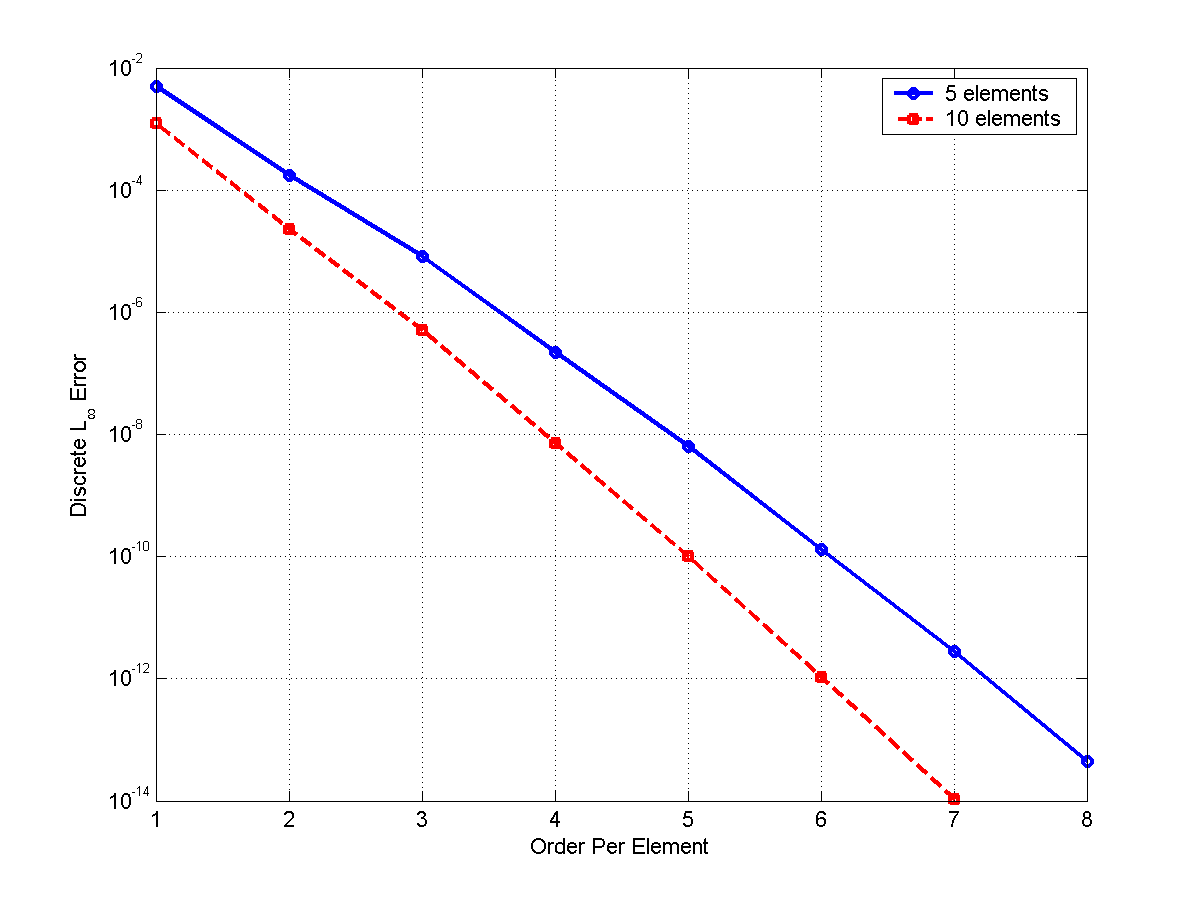
\epsfig{file = figs_dd/sinDDpconv.eps, %
        height = 9cm}
\caption{\label{sinDDpconv}Graph showing change of errors by the
increase of the number of elements: Dirichlet-Dirichlet}
\end{center}
\end{figure}

\begin{table}[h]
\centering \caption{\label{pconv1t} Specification of
                              Figure\ref{sinDDpconv} and their errors}
\begin{tabular}{|c|c|} \hline
Element Size&Error   \\ \hline \hline
    0.2&$7.7716e-016$  \\ \hline
    0.1&$1.1796e-016$  \\ \hline
\end{tabular}
\end{table}

\item Dirichlet-Neumann Case


\begin{figure}[h]
\begin{center}
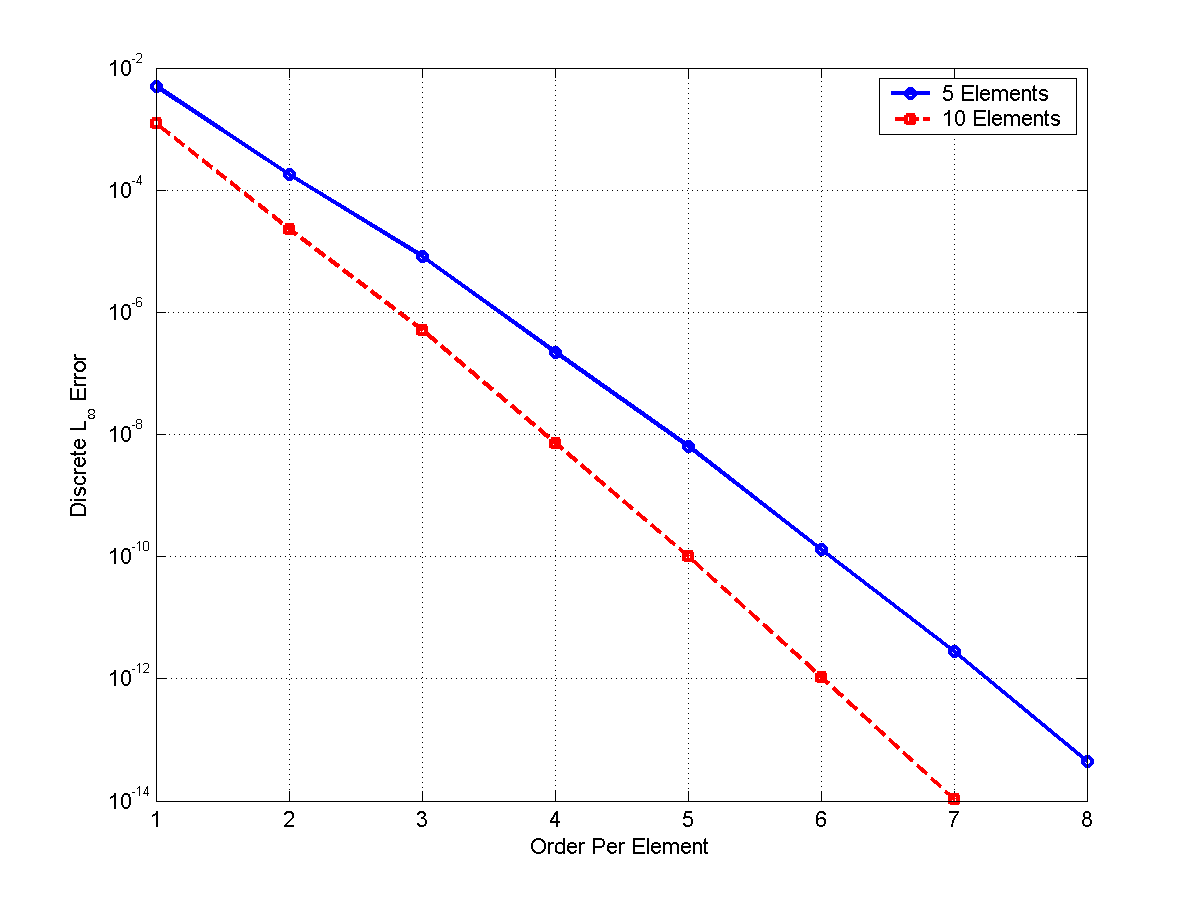
\epsfig{file = figs_dn/sinDNpconv.eps, %
        height = 9cm}
\caption{\label{sinDNpconv}Graph showing change of errors by the
increase of the number of elements: Dirichlet-Neumann}
\end{center}
\end{figure}

\begin{table}[h]
\centering \caption{\label{pconv2t} Specification of
                              Figure\ref{sinDNpconv} and their errors}
\begin{tabular}{|c|c|} \hline
Element Size&Error   \\ \hline \hline
    0.2&$8.3267e-016$  \\ \hline
    0.1&$6.6613e-016$  \\ \hline
\end{tabular}
\end{table}


\end{itemize}
